Механизм STREAMS --- довольно устаревшая вещь. Альтернатива сокетам в System V.

Это модель, которая представляет собой поток, у которого есть некая вершина, набор драйверов и конечное устройство. 

Базовая единица STREAMS - stream, двунаправленный способ передачи данных между процессом в пользовательском пространстве и драйвером STREAMS в ядре. Stream состоит из заголовка, драйвера и N-го количество модулей.

\begin{figure}[htbp]
  \centering
  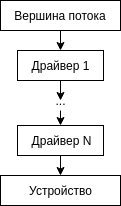
\includegraphics[width=0.15\textwidth]{./processes-and-threads/processes-interconnection/STREAMS/STREAMS.png}
\end{figure}

\textbf{Попробуем привести пример.}

Есть устройство, которое ничего не знает про TCP и UDP, оно знает MAC-адрес получателя и данные. Есть драйвер, который может запаковать IP-адрес в MAC-адрес и запаковать эти данные для сетевого устройства. Драйвер умеет только преобразовывать IP-адрес в MAC-адрес. 

Есть драйвер, который реализует работу с TCP и UDP, но ничего не знает про MAC-адреса, поэтому он подготавливает адреса для драйвера, который ниже. И так всё выше и выше, где есть вершина, которой мы говорим, что хотим отправить данные в таком-то направлении. 

Соответственно наши данные проходят через ряд настроенных нами драйверов. Эти драйвера оборачивают эти данные заголовками и отправляют в устройства. Устройства этот большой пакет отправляют в сеть. 

Модель красивая, потому что одна программа занимается ровно одной задачей. К сожалению, она несостоятельна, потому что постоянно копировать большие объемы данных внутри оперативной памяти даже быстрой всё равно медленно. Поэтому и не используется. 

STREAMS могут быть использованы для:

\begin{itemize}
	\item имплементации сетевых протоколов;
	\item разработки символьных устройств;
	\item разработки сетевых контроллеров (например, карты Ethernet);
	\item ввода-вывода на терминал.
\end{itemize}
